\section{Existujúce riešenia}
\subsection{Mapbox}

\indent \indent \textit{Mapbox} je platforma údajov o polohe pre mobilné a webové aplikácie\cite{mapbox}. Poskytuje mnoho produktov: \textit{Mapbox GL JS} knižnicu, pomocou ktorej je možné vytvoriť interaktívnu, prispôsobenú a efektívnu mapu vo webovej aplikácii\cite{mapbox_gljs}, \textit{Navigation SDK for mobiles}, riešenie pre vytváranie navigácie v mobilných telefónoch dostupné pre \textit{Android} aj \textit{iOS}\cite{mapbox_mobile_navigation},  \textit{MapGPT}, prvého \acrshort{ai} asistenta, s ktorým je možné mať konverzácie ohľadom ciest, navigačných inštrukcií alebo atrakcií\cite{mapbox_mapgpt}. \\
Výhody Mapboxu:
\begin{itemize}
  \item Ponúka 50 tisíc načítaní mapy vo webovej aplikácii.
  \item Poskytuje map-match funkciu.
  \item Prispôsobenie štýlov mapy, markerov alebo vyskakovacích okien.
\end{itemize}
Nevýhody
\begin{itemize}
  \item Trasa sa dá zobraziť až po použití \textit{Mapbox GL JS} a implementovaní vlastnej webovej aplikácie.
  \item Vstupné dáta treba upraviť na požadovaný formát pred odoslaním do \textit{Mapbox \acrshort{api}}.
  \item Do jednej požiadavky na map-match funkciu je možné vložiť len 100 bodov, preto je potrebné pre dlhšie trasy (tisíc bodov a viac) urobiť niekoľko požiadaviek. 
  \item Pri aplikácií, ktorú používa veľa používateľov (rádovo tisíc) dôjde k rýchlemu vyčerpaniu kvóty pre map-match (100 tisíc použití funkcie mesačne zadarmo). 
  \item Rozdelenie trás do viacerých požiadaviek spomaľuje rýchlosť pripínanie trás k cestnej sieti.
  \item Trasa je ku cestnej sieti pripnutá nepresne, viď obrázok \ref{fig:mapbox-map-match-vs-valhalla}.
  \item Je potrebné použiť online \acrshort{api}, čo spomaľuje pripínanie trás k cestnej sieti.
\end{itemize}
\begin{figure}[H]
  \centering
  \begin{subfigure}{.45\textwidth}
    \centering
    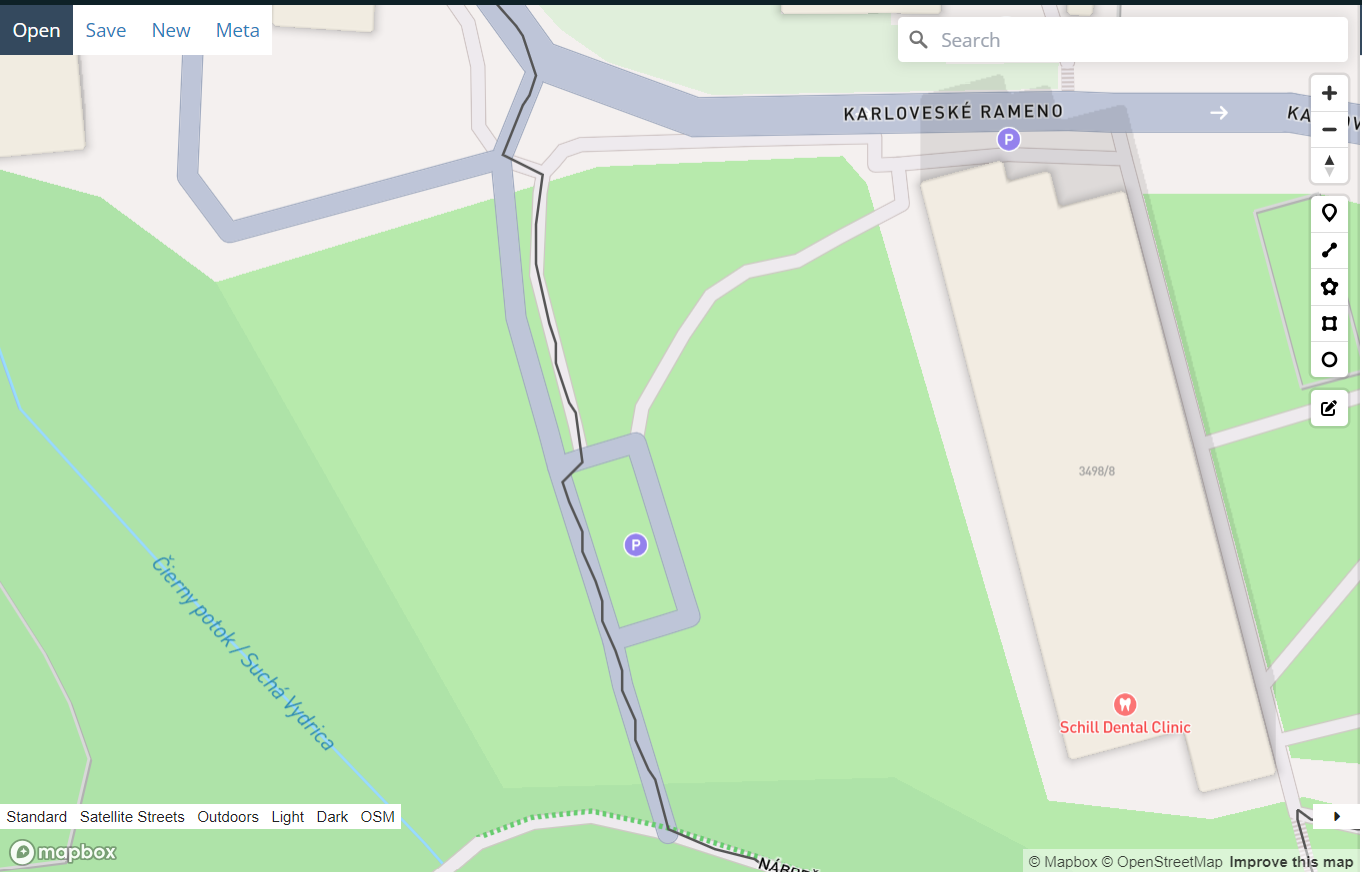
\includegraphics[width=1\textwidth]{img/porovnanie_map_match/mapbox-map-match.png}
    \caption{Map-match od Mapbox}
    \label{fig:mapbox-map-match}
  \end{subfigure}
  \begin{subfigure}{.45\textwidth}
    \centering
    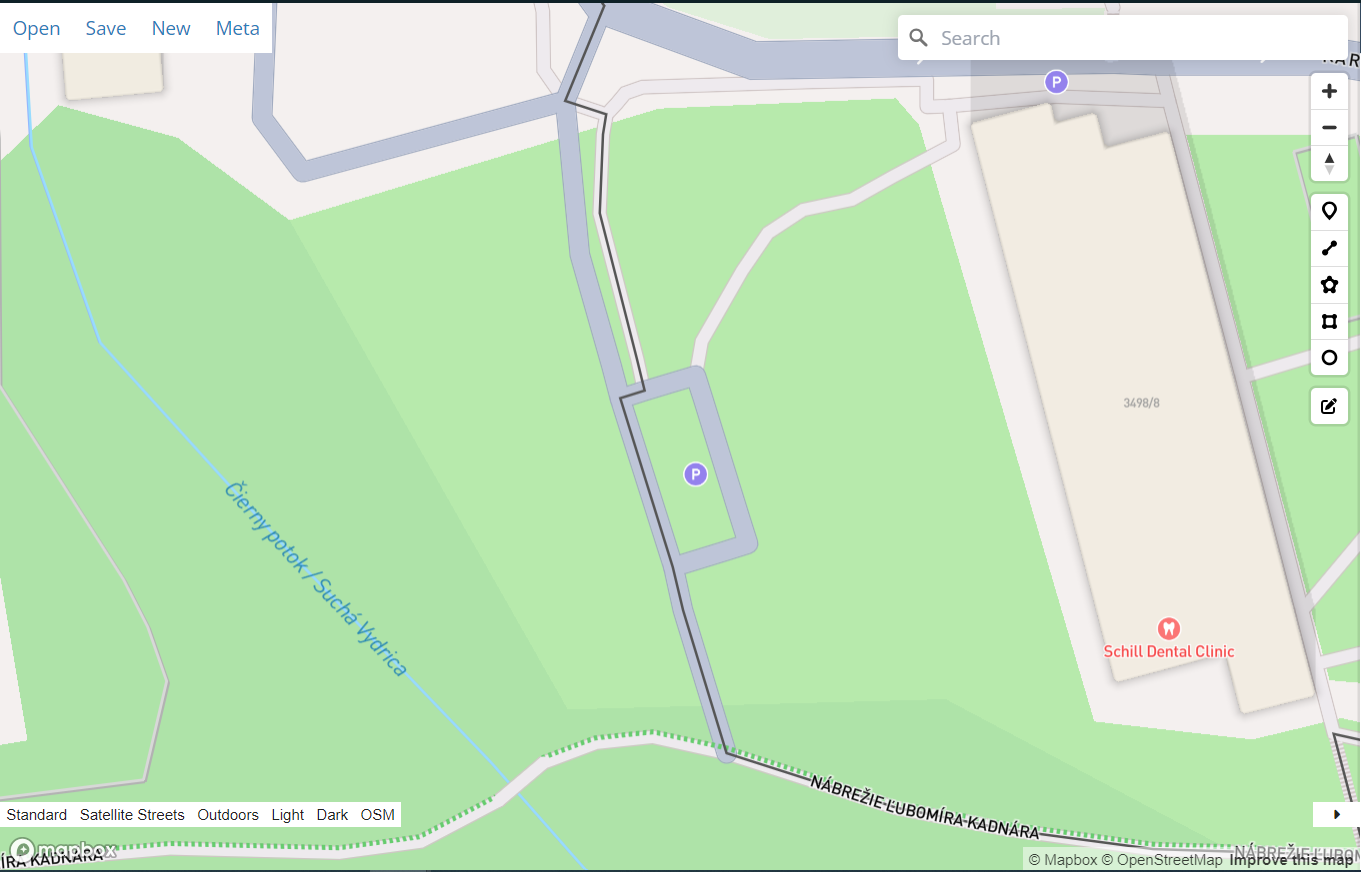
\includegraphics[width=1\textwidth]{img/porovnanie_map_match/valhalla-map-match.png}
    \caption{Map-match od Valhally}
    \label{fig:valhalla-map-match}
  \end{subfigure}
  \caption{Porovnanie Mapbox a Valhalla map-match}
  \label{fig:mapbox-map-match-vs-valhalla}
\end{figure}

\subsection{GPS Visualizer}

\indent \indent \textit{GPS Visualizer} je online nástroj, ktorý vytvára mapy a profily z geografických údajov. Ľahko sa používa, je prehľadný a rýchly. Používateľ pri prvom pohľade na nástroj vie, ako ho používať. Vstup môže byť vo forme údajov GPS (trasy a body na ceste), jazdných trás, ulíc alebo jednoduchých súradníc. Používa sa na zobrazenie trás, plánovanie trasy alebo na rýchlu vizualizáciu geografických údajov (vedecké pozorovania, zobrazenie nehnuteľností, geograficky označených fotografií a podobne). Na webe je od októbra 2002\cite{gps_visualizer}.\\
Výhody:
\begin{itemize}
  \item Rýchly, prehľadný a ľahký na použitie.
  \item Dokáže načítať dáta z rôznych zdrojov (GPX, URL, FIT, CSV, TRK a ďalšie).
  \item Mapu so zobrazenou trasou je možné stiahnuť vo formáte HTML stránky na neskoršie zobrazenie.
\end{itemize}
Nevýhody:
\begin{itemize}
  \item Neponúka map-match, iba zobrazuje trasy.
  \item Pre zobrazenie trasy je nutné zakaždým nahrať súbor s GPS údajmi.
  \item Nutnosť pripojenia na internet kvôli načítaniu knižníc.
\end{itemize}
Prostredie GPS visualizer je zobrazené na obrázkoch nižšie \ref{fig:gps-visualizer}.
\begin{figure}[H]
  \centering
  \begin{subfigure}{.9\textwidth}
    \centering
    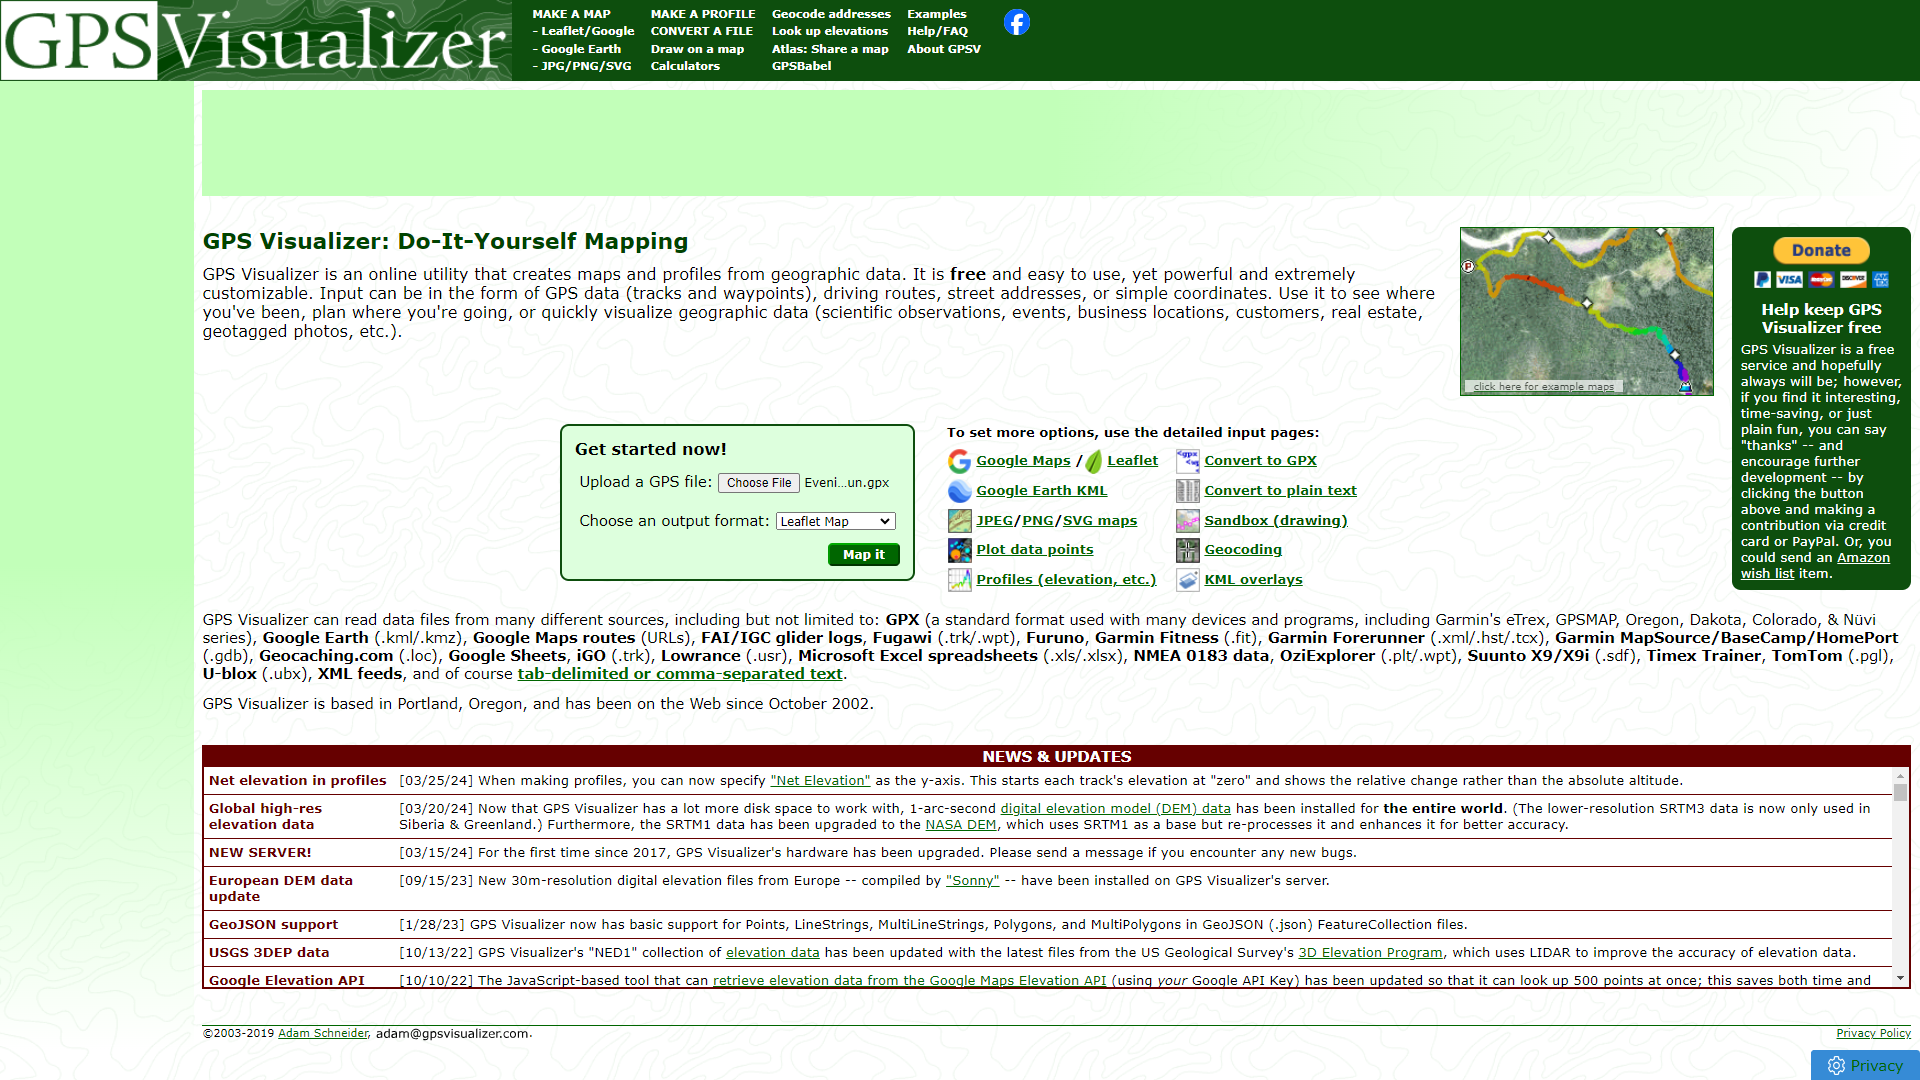
\includegraphics[width=1\textwidth]{img/gps_visualizer/gpsvisualizer1.png}
    \caption{Nahratie trasy}
  \end{subfigure}
  \begin{subfigure}{.9\textwidth}
    \centering
    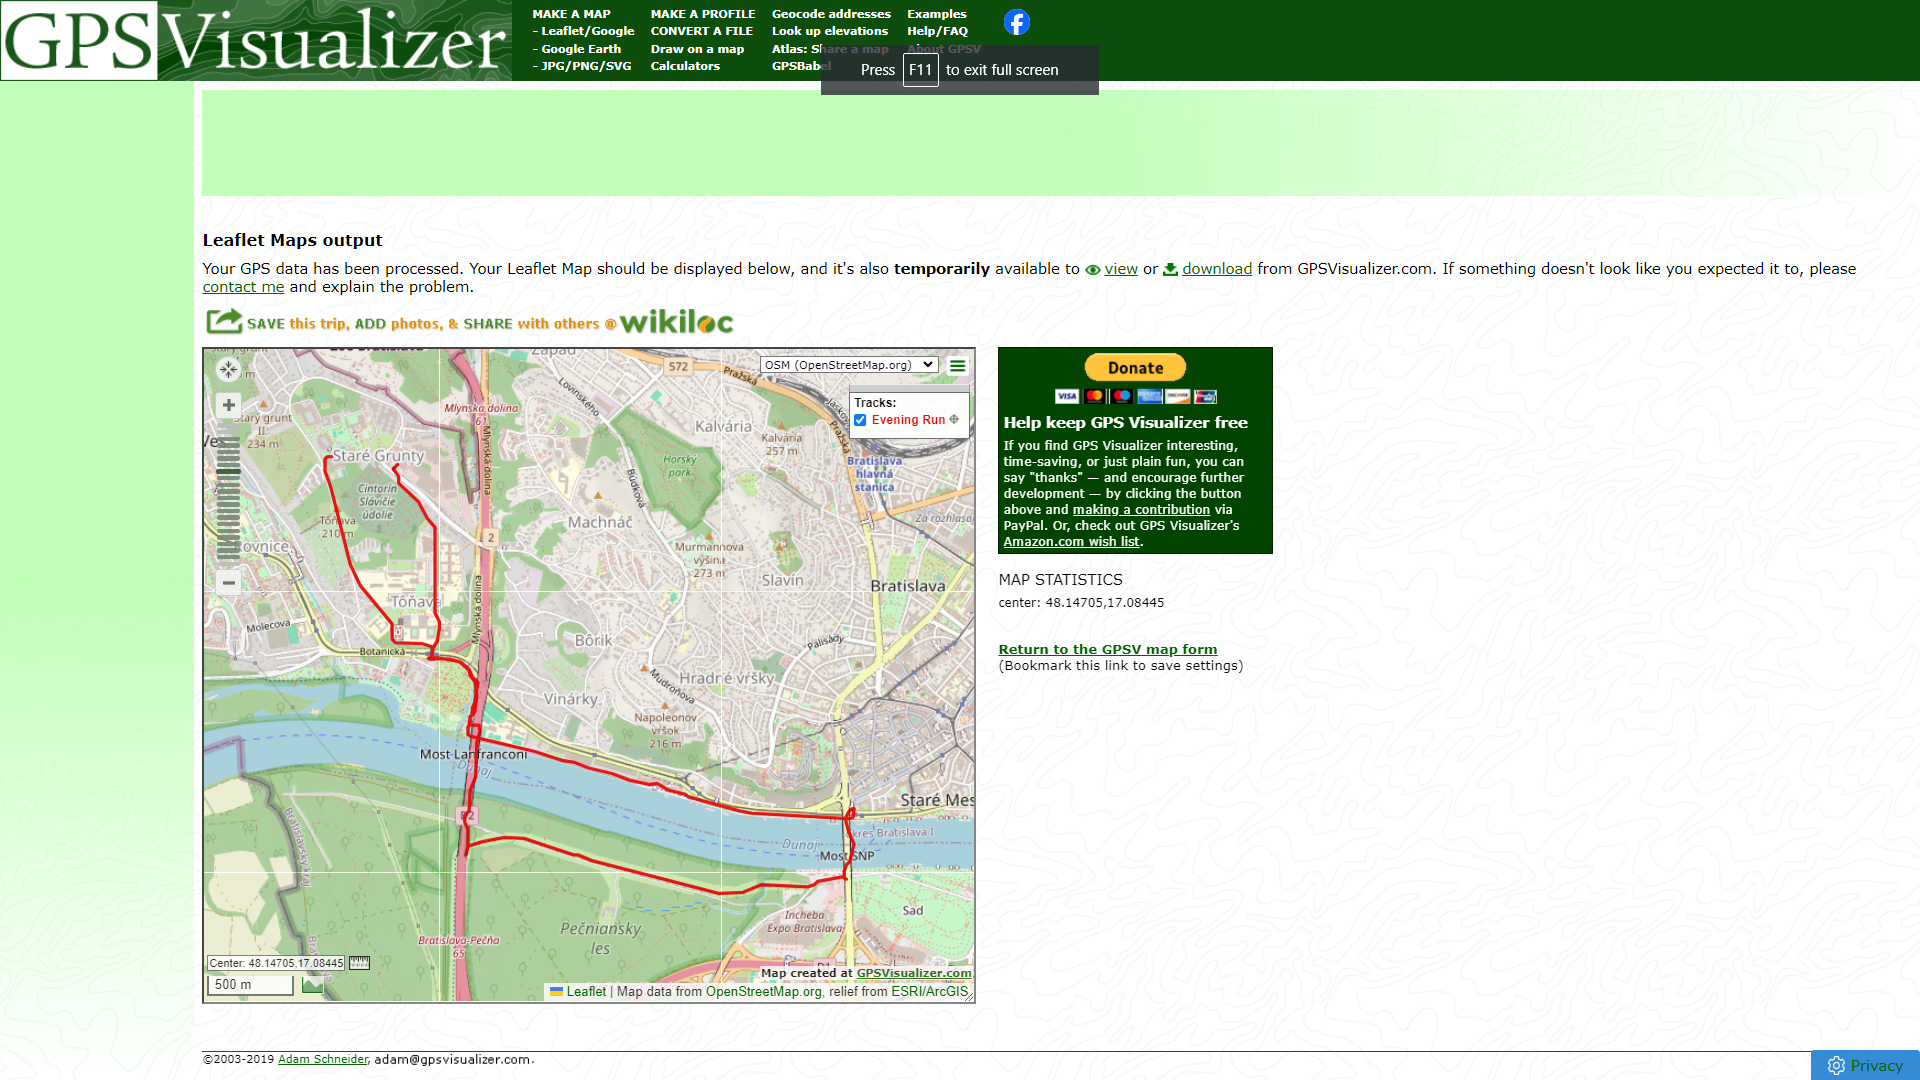
\includegraphics[width=1\textwidth]{img/gps_visualizer/gpsvisualizer2.png}
    \caption{Zobrazenie trasy}
  \end{subfigure}
  \caption{Prostredie GPS Visualizer}
  \label{fig:gps-visualizer}
\end{figure}

